\section{Testen}\label{section:prototypische-implementierung:testen}

\begin{figure}[tbp]
    \centering
    \begin{tikzpicture}
        \begin{class}[text width=6cm]{TestingServiceProducer}{0,0}
            \operation{+ registerFunction()}
            \operation{+ onStartTesting()}
            \operation{+ onEndTesting()}
            \operation{+ onFunctionCall()}
        \end{class}
        \begin{class}[text width=6cm]{TestingServiceConsumer}{7,0}
            \operation{+ addTest()}
            \operation{+ runTest()}
            \operation{+ startTesting()}
            \operation{+ endTesting()}
        \end{class}
    \end{tikzpicture}
    \caption{Klassendiagramm Testing Service}
    \label{figure:klassendiagramm-testing-service}
\end{figure}

Für die prototypische Implementierung wurde der in \autoref{section:konzeption:testen} konzipierte Testing Service implementiert. Das Klassendiagramm für diesen kann in \autoref{figure:klassendiagramm-testing-service} eingesehen werden. Der Testing Service Producer ermöglicht es Laborgeräten mithilfe von \texttt{registerFunction()} Funktionen für die Erstellung von Testfällen bereitzustellen. Dabei sollten neben dem Namen und der Implementierung der Funktion auch Schemata für die Argumente und den Rückgabewert der Funktion angegeben werden, damit eine Validierung dieser möglich ist. Die Erstellung von Testfällen kann während der Erstellung eines Experiments vorgenommen werden. Dabei werden diese in der Konfiguration des Laborgeräts hinterlegt, welches den Testing Service Consumer anbietet. Der Testing Service Consumer kann, wie in der Konzeption beschrieben, mit \texttt{startTesting()} das Testen starten, mit \texttt{runTest()} Testfälle ausführen und mit \texttt{endTesting()} das Testen beenden. Der Testing Service Producer löst entsprechende Events aus, die über Event-Handler behandelt werden können.

\begin{figure}[tbp]
    \centering
    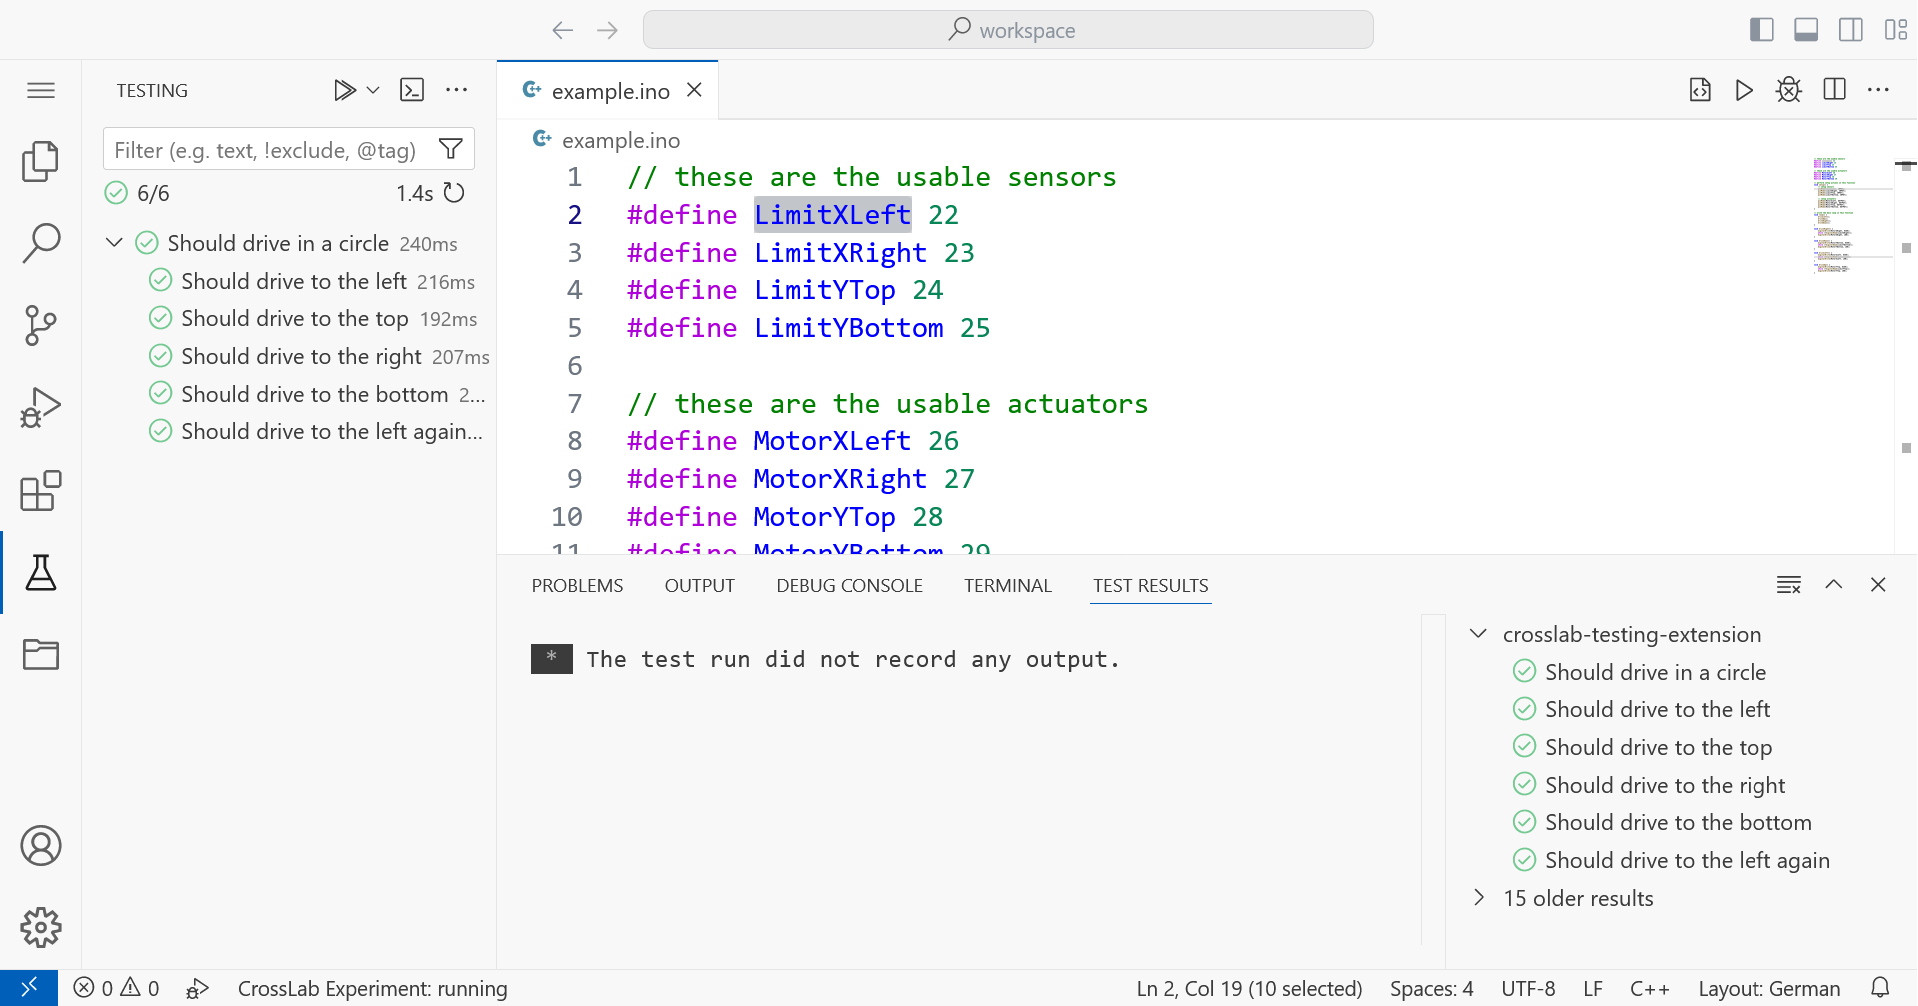
\includegraphics[trim={0 3px 0 0},clip,width=\textwidth]{images/tests-success.png}
    \caption{Benutzerinterface für die Ausführung von Testfällen}
    \label{figure:benutzerinterface:testen}
\end{figure}

Für die IDE wurde eine entsprechende Erweiterung implementiert. Diese wird im Folgenden als \textit{Testing Erweiterung} bezeichnet und stellt einen Testing Service Consumer bereit. Weiterhin wird die VSCode Testing API, ein Teil der VSCode Extension API, verwendet, um die Testfälle in der IDE anzeigen und ausführen zu können. Dabei wird das bereits in VSCode enthaltene Benutzerinterface für Tests verwendet. Dieses ist in \autoref{figure:benutzerinterface:testen} dargestellt.

Der betrachteten Experimentkonfiguration wird kein neues Laborgerät hinzugefügt. Jede IDE wird um einen Testing Service Consumer und die Steuereinheit um einen Testing Service Producer erweitert. Zudem stellt die Steuereinheit Funktionen zum Setzen und Auslesen der Pins des simulierten Microcontrollers zur Verfügung. Es werden Verbindungen zwischen den IDEs und der Steuereinheit über den Testing Service hinzugefügt (siehe \autoref{figure:experimentkonfiguration:testen}).